\todo[backgroundcolor=orange]{SEC: Definition of a Network}
Community detection relies on us knowing lots about the underlying structure of a network and to do that we have to understand its properties. This chapter will establish a more formal understanding of networks and will highlight some key properties and methods that we will use to exctract value about community structure later.

\begin{definition}{(Undirected network)}
    Let $V$ be a set of vertices (nodes) and let $E$ be a set of pairs of vertices such that if $e = (x, y) \in E$ then $x, y \in V$. An undirected network is the pair $(V, E) = N$. An edge $e = (x, y) \in E$ is said to join $x$ and $y$ and $y$ to $x$.\cite[1]{oxford:renaud_notes}\label{def:undirected_network}
\end{definition}

The undirected network is the simplest type of network and on its own has interesting enough properties. However, for the sake of example and application, we will also introduce some other types of network that allow for more detailed models.

\todo[backgroundcolor=orange]{SEC: Different Types of Network}

\begin{definition}{(Directed network)}
    Let $V$ be a set of vertices (nodes) and let $E$ be a set of pairs of vertices such that if $e = (x, y) \in E$ then $x, y \in V$. A directed network is the pair $(V, E) = N$. An edge $e = (x, y) \in E$ is said to join $x$ to $y$. I.e. if $x$ is joined to $y$ then $y$ is not necessarily joined to $x$.\cite[1]{oxford:renaud_notes}\label{def:directed_network}
\end{definition}

The intuition for directed graphs, is that edges may only be travelled along in one way. This comes in handy for modelling more intricate systems. The final network type of interest is that of the weighted network.

\begin{definition}{(Weighted network)}
    Let $V$ be a set of vertices (nodes) and let $E$ be a set of triples of the form $V^2 \times \mathbb{R}$ such that if $e = (x, y, w) \in E$ then $x, y \in V$. The value $w$ is said to be the weight of the edge.\cite[1]{oxford:renaud_notes}\label{def:weighted_network}
\end{definition}
\todo[backgroundcolor=orange]{SEC: Interesting Properties of Networks}

The weighted network allows us to introduce some notion of how hard it is to move along a certain edge. This is useful when modeling things like traffic flow. [citation needed]

The above definitions of a network are likely more technical than we will ever need because once we have introduced the notion of of an adjacency matrix, that becomes our go to representation of a network.

\subsection{Adjacency Matrices}
The objects defined above are meaningless without a concrete way of mathematically representing them. To that end, we have to come up with a way of describing a network mathematically. This leads us to the definition of the adjacency matrix:

\begin{definition}{(Adjacency matrix)}
    Let $N = (V, E)$ be a network and label every vertex $v \in V$ with a number from $1$ to $n = |V|$. The adjacency matrix of a network is the matrix of elements $(A)_{ij}$ such that $a_{ij} = 1$ if $(i, j) \in E$ and $a_{ij} = 0$ if $(i, j) \notin E$. In other words, if nodes $i$ and $j$ are connected by an edge in the network, then the corresponding element in the matrix is $1$. Otherwise, it is $0$.\label{def:adjacency_matrix}
\end{definition}

\begin{figure}
    \begin{center}
        \begin{subfigure}[b]{0.45\textwidth}
            % 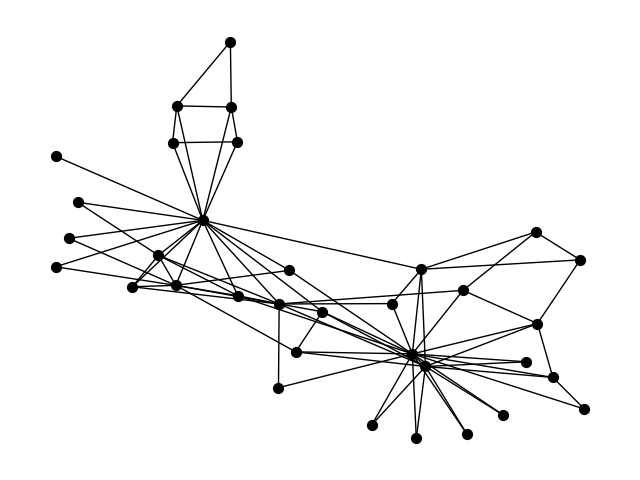
\includegraphics[width=\textwidth]{img/zachary_spring}
            \missingfigure{Simple graph}
            \caption{Simple graph}
            \label{fig:simple_network}
        \end{subfigure}
        \begin{subfigure}[b]{0.45\textwidth}
            % 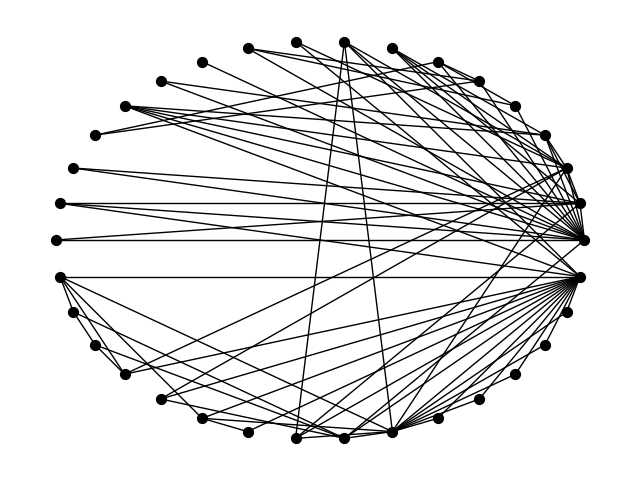
\includegraphics[width=\textwidth]{img/zachary_circle}
            \missingfigure{Adjacency matrix of simple network}
            \caption{Adjacency matrix}
            \label{fig:simple_network_adjacency_matrix}
        \end{subfigure}
    \end{center}
    \caption{A simple network and its adjacency matrix}
    \label{fig:simple_network_and_adjacency_matrix}
\end{figure}

The adjacency matrix gives us our first way of representing a network. Figure \ref{fig:simple_network_and_adjacency_matrix} shows a basic example of a network and its associated adjacency matrix. This will form the basis for most of the analytical work we do going forwards. It's worth noting that there are also different types of adjacency matrix corresponding to the different types of network. For example, in the case of a directed network we will have a non-symmetric matrix where $a_{ij} = 1$ if $(i, j) \in E$ but this does not necessarily mean that $a_{ji} = 1$. We also get something similar for weighted networks where we set $a_{ij} = w$ the weight of the edge connecting $i$ and $j$ in $N$.

\subsection{Bipartite Graphs}
Not really sure if it's worth talking about these.

\subsection{Paths}
When we're analysing a network, we're very often interested in which vertices are reachable from any given vertex. As such, we become interested in the idea of a path. A path in a network is defined in the following way

\begin{definition}{(Path)}
    Let $N = (V, E)$ be a network. A path is a sequence of distinct vertices $v_1, \dots, v_n \in E$ such that $(e_i, e_{i+1}) \in E$ for all $i = 1, \dots, n-1$. In other words, a path is a sequence of distinct vertices such that every consecutive pair of vertices is connected by an edge in $E$.
\end{definition}

Paths are an important concept in community detection as they allow us to phrase questions in rigorous terms as opposed to loose concepts of connectedness.

\subsection{Components}

\subsection{Cut Sets}

\subsection{The Graph Laplacian}
